%\vspace*{-80mm}
\chapter{Introduction}
\label{sec:introduction}
%\section{\sloppy Software Obfuscation}
% Software Obfuscation is an important cryptographic concept with wide applications.However until recently there\cite{Sen}
% was little theoretical investigation of obfuscation, despite the
% great success theoretical cryptography has had in tackling
% other challenging notions of security\cite{lynn2004positive}. 

% Usually we would like our source codes to be readable while software obfuscation research does exactly the opposite process which harden the understanding process or make it even impossible. 
% The final goal of conducting
% software obfuscation is to hide those classified or sensitive
% information which could be extracted by some reverse engineering means and  at the same time preserving software’s functionality. We can always treat obfuscation method as a virtual
% black box or a compiler which could transform the primitive
% source code to instrumented codes that will behave exactly
% the same as the original codes. Which means, the obfuscated programs will yield outputs the same with the original out-
% puts given identical inputs.\cite{TuringmachineSimulation}




% %%%
% \begin{figure}[htb]
%     \centering
% %    \includegraphics{\FigPath{FigureFileName}}
%     \caption{CaptionText.}
%     \label{ChX-figure: FigureLabel}
% \end{figure}
% %%%

% \subsubsection{Obfuscation Benefits}
% There are many reasons to obfuscate source codes. Software obfuscation could help companies or individuals protect their intellectual property from being theft. With the development of distributed system and cloud computing, more and more users begin to store data on public web services like Amazon Web Service, it induces privacy leak risk which would do huge damage to Internet community if not dealt properly. Obfuscation could exert great  influence on protect end users' privacy. Another big battle filed of software obfuscation is to compete with the dark side of the software security - Hackers. Hackers do a lot harm to the world exploiting vulnerabilities of software every year. On important step to hack victims' system is to reverse engineer the software binaries and figure out the logic of it. Although an experienced hacker could always reverse engineer a software given enough time and energy, software obfuscation could make this extremely hard.


% \section{Obfuscation Research Situation}
% In early days, most obfuscation protection systems encrypt the code and then decrypt it at the application's startup. This method is easy to implement while it is also risky and could be easily deobfuscated if an hacker figured out the encryption algorithm.




<<<<<<< HEAD
% \subsubsection{Negative Integer Operand Preprocess}
% % what if 4 + (-6)?  would you translate it into 4 + 6?
% \textcolor{red}{still not clear}
% In software programs, integer operands comprise both positive and negative
% cases. Turing machine could only dispose of positive operands in consequence of
% we use the length of dot cell on tape to represent a integer. This means we have
% to preprocess the invalid operands in Turing machine obfuscator. In the
% preprocessing stage, Turing machine obfuscator could convert invalid operands to
% its opposite number to run Turing machine. Calculate result from Turing machine
% is also revised before returning. For instance, $-4 + (-6)$ is preprocessed to
% $4 + 6$, afterwards -10 which is the opposite number of 10 is returned. $4 +
% (-6)$ is preprocessed to Turing machine operation $6 - 4$, and the opposite
% number of the outcome 2 (i.e., -2) is returned. In preprocess stage, any
% arithmetic operation would be transformed to a valid integer operation with $+$,
% $-$, $\times$, $\div$ for Turing machine.

% Formally a Turing machine could be represented by a 7 element tuple\cite{Turing}: \[ (Q, \Gamma, b, \Sigma, \delta, q_0, F) \] 
% where:
% \begin{itemize}
%   %\renewcommand{\labelitemi}{$\star$}
%   \item \(Q\) is finite state set
%   \item \(\Gamma\) is finite tape symbol set named alphabet
%   \item \(b\) is the tape blank symbol. \(b \in \Gamma\)
%   \item \(\Sigma \subset \Gamma \)\textbackslash  \(\{b\}\) is the actual input symbol set without blank symbol
%   \item \(\delta\) is the transition table composed of transition rules in form of \((Q\)\textbackslash \(F)\times\Gamma \rightarrow Q \times \Gamma \times \{L,R\}\) 
%   \item \(q_0 \in Q \) is the initial state
%   \item \(F\) is finite acceptable states set. \(F \subset Q\)
% \end{itemize}




Obfuscation is an important technique for software protection.
Attackers could take advantage of the
state-of-the-art techniques~\cite{Loop,Lee,Molnar} to recover program source or high-level
code from executables, exploit software vulnerabilities, and steal algorithm
implementations. Software obfuscation is mostly designed to impede such
(malicious) reverse engineering process. It is also used by malware developers to
hide their malicious intent.

Recently, software security has drawn more and more attention because of, for example,
infamous ransomware attacks and severe vulnerabilities such as the ``WannaCry''
incidence~\cite{wannacry} and the OpenSSL ``Heartbleed'' bug~\cite{Heartbleed}. All of
these malware programs exploit vulnerabilities inside a program. To launch such attacks,
attackers usually need to recover the control flow structures of the victim
programs first. Symbolic execution and concolic testing are 
widely-adopted techniques to cover execution paths and explore program
structure~\cite{dart,exe,Sen,symbol}. Typical symbolic execution engines such as
SAGE~\cite{Sage} and KLEE~\cite{klee} could yield new input which leads to a new
execution path by solving branch conditions  with a constraint
solver. After all execution paths are traversed, control flow graph of the program could be restored
with the traversing information.
Such tools have been proven to be very effective in analyzing program
control flow structures~\cite{Cute}.

Hence, a lot of anti-reverse engineering research has focused on preventing
adversaries from analyzing important path conditions in a
program~\cite{Opaque,Sharif,Popov,Zhi, Wang:Zhi}. Control flow obfuscation is
one of these cutting-edge techniques to combat these reverse engineering tools.
Control flow obfuscation aims at hiding path conditions and complicating the
execution flow within a program. By rewriting or adding extra control flow
components, the program path conditions become difficult or even impossible to
analyze. Existing research~\cite{Ma} have demonstrated the effectiveness of
control flow obfuscation.

% \begin{figure}
%   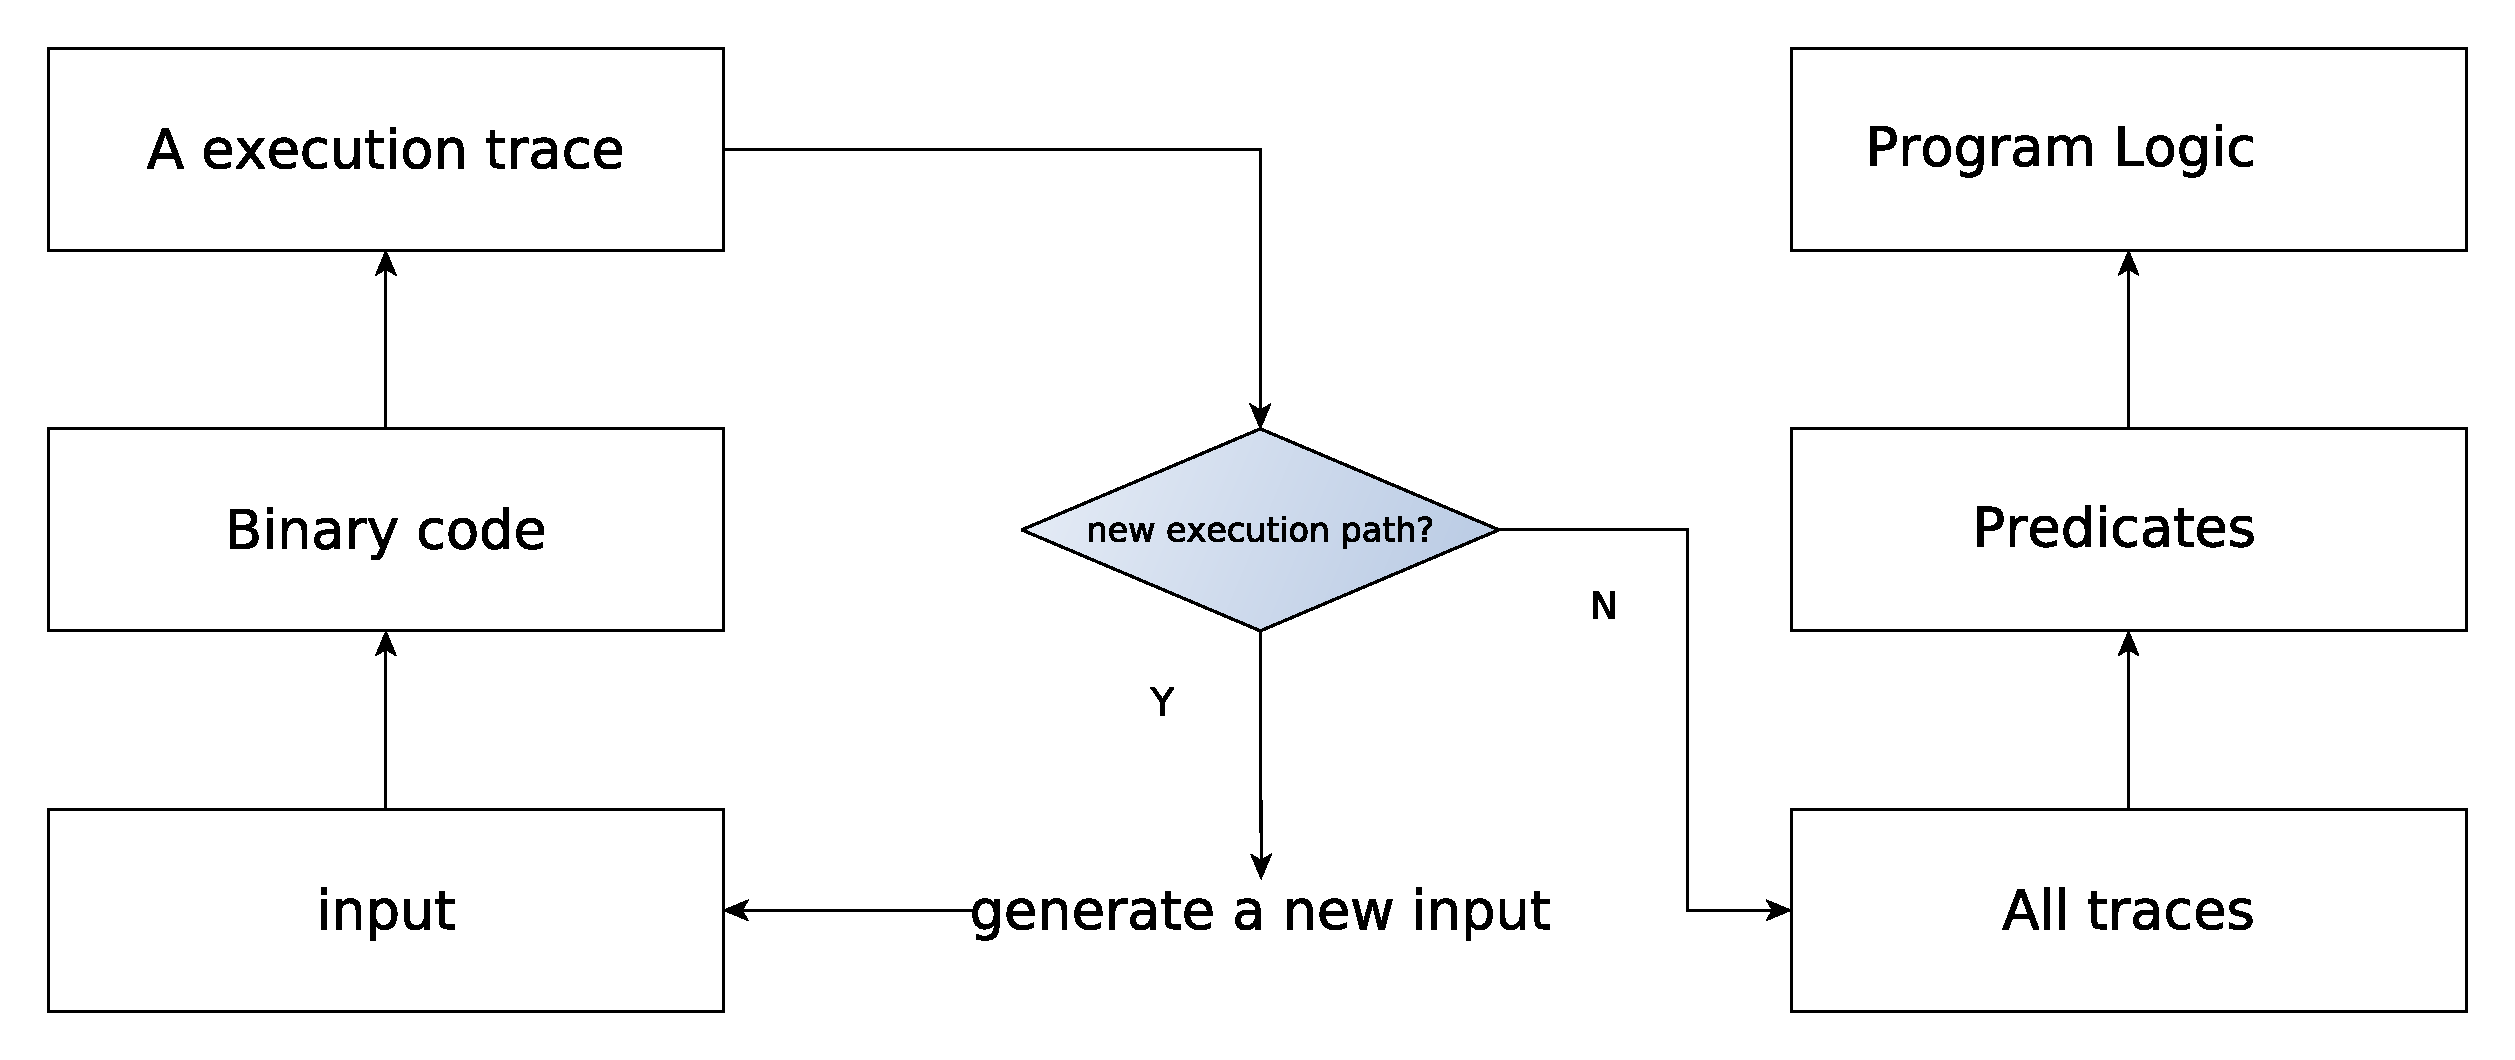
\includegraphics[width=0.9\linewidth]{reverse_engineering.eps}
%   \caption{Reverse engineering with concolic testing}
%   \label{fig:one}
% \end{figure}

In this thesis, we propose a novel control flow obfuscation method which
leverages Turing machine to compute path conditions. The \textit{Church-Turing
  thesis}~\cite{Church} states that the power of Turing machines and
$\lambda$-calculus is the same as algorithms, or the informal notion of
effectively calculable functions. Formally, Turing computable,
$\lambda$-computable, and general recursive functions are shown to be
equivalent, and informally, the thesis states that they all capture the power of
algorithms or effectively calculable functions. This means any functional
component of software can be re-implemented as or transformed into a Turing
machine; the replaced code component and its corresponding semantic equivalent
Turing machine is called \textit{Turing Equivalent}.

Our method is to simulate important branch condition statements in a
program with semantically equivalent Turing machines. A Turing machine
behaves as a state machine so it would bring in a large amount of extra control
flow transfers and basic blocks to the overall program control flow graph.
Moreover, a typical Turing machine leverages a transition table to guide the
computation, and such transition table-based execution would introduce
additional computations and make the overall execution flow much more
complicated. We envision the proposed technique would largely complicate the
protected program, and also bring in new challenges for reverse engineering
tasks. Our method can also be used to obfuscate other computation as well.

To obfuscate a program through the proposed Turing machine obfuscation
technique, we first translate the original program source code into a compiler
intermediate representation. Our Turing machine obfuscator then selects branch
condition statements for transformation; the transformed instructions will invoke its
corresponding Turing machine component, which is semantically equivalent to the
original branch condition. After finishing the execution in the Turing machine
``black box'', the execution flow returns back to the original instruction, with
a return value which determines the branch selection. Inspired by previous
work~\cite{Collberg}, we evaluate our obfuscator regarding five aspects which
are functionality correctness, potency, resilience, cost, and stealth. Results
indicate that Turing machine obfuscator could effectively obfuscate
commonly-used software with acceptable cost and robustness.

This thesis is organized as follows. Section 2 discusses related works on
obfuscation, especially control flow obfuscation. Section 3 presents the overall
design of Turing machine obfuscator. Obfuscator implementation is discussed in
Section 4. Section 5 presents the evaluation result of our proposed technique.
We further present discussion in Section 6, and conclude the theis in Section 7.



In Turing machine obfuscator, we collect all comparison instructions for branch
predicate instructions (e.g., \texttt{icmp}). Through use-def chain analysis,
we also locate all instructions that determine the value of the conditional
branch instruction, all these instructions are deemed as transformation
candidates.
=======
\subsubsection{Negative Integer Operand Preprocess}
% what if 4 + (-6)?  would you translate it into 4 + 6?
\textcolor{red}{still not clear}
In software programs, integer operands comprise both positive and negative
cases. Turing machine could only dispose of positive operands in consequence of
we use the length of dot cell on tape to represent a integer. This means we have
to preprocess the invalid operands in Turing machine obfuscator. In the
preprocessing stage, Turing machine obfuscator could convert invalid operands to
its opposite number to run Turing machine. Calculate result from Turing machine
is also revised before returning. For instance, $-4 + (-6)$ is preprocessed to
$4 + 6$, afterwards -10 which is the opposite number of 10 is returned. $4 +
(-6)$ is preprocessed to Turing machine operation $6 - 4$, and the opposite
number of the outcome 2 (i.e., -2) is returned. In preprocess stage, any
arithmetic operation would be transformed to a valid integer operation with $+$,
$-$, $\times$, $\div$ for Turing machine.
>>>>>>> e49a644b666da86f78dcd082fd52d1c6d25a270f
